\documentclass{cslthse-msc}
\usepackage[utf8]{inputenc}
\usepackage[english]{babel}
\usepackage{amsmath}
\usepackage{amsfonts}
\usepackage{amssymb}
\usepackage{amsthm}
\usepackage{makeidx}
\usepackage{graphicx}
\usepackage{multirow}
\usepackage{listings}
\usepackage[titletoc, header, page]{appendix}
%for line break in url
\usepackage{hyperref}
%line break in compiled document for line break in tex documents
\usepackage{parskip}
\usepackage[nopar]{lipsum}
\usepackage{color}
%for drawing figures
\usepackage{tikz}
% for the web and mobile app with backend figures
\usetikzlibrary{arrows,positioning}

\definecolor{mygreen}{rgb}{0,0.6,0}
\definecolor{mygray}{rgb}{0.5,0.5,0.5}
\definecolor{mymauve}{rgb}{0.58,0,0.82}

\lstset{
	basicstyle=\footnotesize,
	language=Java,
	keywordstyle=\color{blue},
	commentstyle=\color{mygreen} 
	}

% to highlight with a black rectangle when a overfull hbox occurs to make it easy to spot
\overfullrule=2cm
%\geometry{showframe}
%\author{
	David Norrestam \\
	{\normalsize \href{mailto:davidnorrestam@gmail.com}{\texttt{davidnorrestam@gmail.com}}}
	\and
	Philip Burenstam Linder \\
    {\normalsize \href{mailto:philip.burenstam.linder@gmail.com}{\texttt{philip.burenstam.linder@gmail.com}}}
}

\title{Hybrid app-development using an existing web application}
%\subtitle{A feasibility study}
\company{Lund University}

%\date{\today}
\date{Month Day, 2015}

\supervisors{Flavius Gruian, \href{mailto:Flavius.Gruian@cs.lth.se}{\texttt{Flavius.gruian@cs.lth.se}}}{Albin Willman, \href{mailto:albin.svensson@trialbee.com}{\texttt{albin.svensson@trialbee.com}}}
%\supervisor{John Deer, \href{mailto:jdeer@company.com}{\texttt{jdeer@company.com}}}
\examiner{Flavius Gruian, \href{mailto:flavius.gruian@cs.lth.se}{\texttt{flavius.gruian@cs.lth.se}}}


\acknowledgements{
We wish to offer our thanks to Trialbee for giving us the idea for this investigation and our supervisor Albin Willman who guided us and helped us develop the web application.

We would also like to take this oppurtunity to thank our examiner, Flavius Gruian at the Department of Computer Science, for all the advices and feedback he has provided throughout the process of writing this thesis.

\theabstract{
Mobile applications are today an important way for companies to reach their customers. Developing a mobile application could require a lot of resources, especially if the application is to be made from scratch. However, an alternative for a company with an existing web application, is making use of the logic in the existing web application, to create a hybrid mobile application.

In this thesis, two different approaches to developing an Android application were evaluated. The application to be developed consisted of classes for communication with native Android functions, and an encapsulated (existing) web application, making use of the functions provided by the aforementioned classes to extend its functionality. In one of the approaches, Android Framework was used for developing the hybrid application, and in the other approach, PhoneGap framework was used.

For evaluation, we recorded the development effort required in each of the two approaches, for a quantitative comparison, and also examined the structure of the developed applications, for a qualitative comparison. Development effort was estimated by measuring logical lines of code (LLoC) of the resulting application. 

The results show that a lower development effort is required when developing using PhoneGap framework, than in the Android framework. However, we noticed that developing using Android framework provides more control over the application life cycle, and can thus be a preferable option when a more advanced application needs to be developed.
}

\keywords{android, hybrid, phonegap, mobile application, web application}

%% Only used to display font sizes
\makeatletter
\newcommand\thefontsize[1]{{#1 \f@size pt\par}}
\makeatother
%%%%%%%%%%



\begin{document}
%\makeFrontMatter
%\chapter{Introduction}
Imagine a smaller company with a well developed web application. The company has a few developers and has the want to extend their web applications features for their users. They want to track their users activity for making a health profile. To track the user's activity they need to use the mobile accelerometer. The accelerometer can be accessed through a mobile application but not through a web application. 

The company can choose to develop a mobile application from the ground up and integrate the application with their current web application. That will cost them a huge amount of development time and also a lot of time maintaining several platforms.

Another less costly alternative is to create the mobile application using the existing web application. The web application is run within a shell of the mobile application. The web application can then access the mobile’s native functions such as the accelerometer. This will save the company time developing the mobile application and instead of maintaining several platforms for every feature the mobile application only need to be maintained in regards of the use of the accelerometer. 

The aim of this thesis is to evaluate two different development methods for encapsulating an existing web application in a mobile application to utilize native functions. With focus on evaluating development and maintenance costs.


\section{Background}
Android is an operating system used on a wide range of devices. For example a mobile device or tv device. Developing Android applications are written in the programming language Java. 

A hybrid application is a native application which is partially written with web technologies. I.e HTML5, CSS and JavaScript. The part of the application written with web technologies runs within a browsers engine in a so called WebView. A web application running in a browser does not have access to a device native functions such as the bluetooth. However a website running within a WebView can through interaction with the application's native code access a device native functions.

PhoneGap is a framework for developing mobile applications. The code is written with web technologies. The code can be compiled to different platforms, such as Android or IOs specific code. The resulting application is a hybrid application. An example of a mobile application built in PhoneGap is Wikipedia's mobile application.  

\section{Terminology}
\begin{description}
  \item[Mobile application] \hfill \\
    Refers to the application being developed, excluding code loaded from remote websites.
  \item[Web application] \hfill \\
    If nothing else is specified it refers to the client-side of the web application.
  \item[Development methods] \hfill \\
    Refers (in the context of this paper) to the methods of mobile application development methods being evaluated. I.e developing the mobile application with PhoneGap or natively in Android.
  \item[Native function] \hfill \\
     A hardware function which a device has. Lets say a mobile has a camera and an accelerator. When writing software for that mobile there are functions to interact with the camera and accelerator. Those functions are called native functions.
\end{description}

\section{Problem formulation}
The goal of this project is to evaluate two different development methods for encapsulating an existing web application in an Android mobile application. The purpose of the mobile application is to give the web application access to the mobile's native functions. An example of such a native function would be accessing the mobile's accelerometer. It is important that the logic of the web application can be written in a general way (non-platform dependant) adapting to the device accessing the web application. So that the same web application code is used for the web application and mobile application.

Antoher goal is that the mobile application only provides data from native functions. In order to achieve that the web application and mobile application should have a master slave relationship. Where the web application acts as the master and the mobile application as the slave. To get data from the mobiles native functions the web application asks for the data and the mobile application passes the data back. 

To limit the scope of the research the development methods is only evaluted for the mobile operating system Android. Android was choosen since it is the most widely used today for mobiles. 

There are two development methods of creating an Android application that will be evaluated. The first development method, the mobile application will be built natively in Android. As the second method, the mobile development framework PhoneGap will be used. The methods will be evaluated and compared from a developers perspective, with the preconditions defined section \ref{section-preconditions}.

\subsection{Preconditions} \label{section-preconditions}
The study is done from a company's perspective and is based on the following prerequisites:
\begin{itemize}
\item There are only a few developers, three or less.
\item There is already an existing web-application that is to be used by the mobile-application.
\item The company has a need and/or desire to extend the functionality of it's web-application with native functions.
\end{itemize}

When examining the methods, the focus has been restrained to the following developing aspects:
\begin{itemize}
\item Development time.
\item Maintainability when the application has been created. 
\item Programming productivity when the application has been created.
\end{itemize}

\section{Litterature study}
Source lines of code is a measurement tool for software development. Source lines of code, also abbreviated as SLOC, is very easy to obtain and is a fairly accurate predictor of development effort\cite[p.~63]{galorath2006}. Measuring SLOC simply means you count the number of lines of code. There are many different ways to measure SLOC, such as Halsted’s approach, function points, physical SLOC and Logical SLOC. 

Physical SLOC is the length of the code excluding comments and blanks. Function points measure functionality and can therefore be measured before the design and coding if the requirement specification complete\cite[p.~187]{galorath2006}. Halsted’s uses measurable properties such as operands and operators and uses them to identify properties of software. Such as the length of the program, difficulty and effort\cite[p.~345]{fenton2015}. Fenton and Bieman describes Halstead’s software science measures as a confused and inadequate measurement. Particularly for other attributes then size.

Logical SLOC measures the number of statements that carry over one or more physical lines.  For languages with terminators this can be done more easily and quickly. As an example, in Java you could count the logical SLOC by counting the number of line-terminating semicolons and closing curly brackets. Logical SLOC represents the programming instructions and data declarations which are converted into executable instructions, i.e. the implementation of the software design. Another positive aspect of of logical SLOC is that it better handles differences in formatting and style conventions than physical SLOC\cite[p.~155]{galorath2006}.

To compare size between two different languages a size conversion table can be used. The table can be used to estimate how many SLOC a program coded in one programming language would have in another language. In the table constructed by Galorath and Evans you can compare a third generation language, a fourth generation language, Ada, Assembly or Pascal\cite[p.~163]{galorath2006}. A third generation language compared to another third generation language would have no conversion rate. 

\section{Contribution statement}
Throughout this work we have been working together very closely. We have reviewed and improved each others work continuously. During development we often been pair programming. With that said we can attribute parts of our work to one of us more then the other. Even though most of the work has been created together. 

Philip designed the code of the web application and the mobile application built natively in Android. David designed the code for the PhoneGap application. David researched different techniques for the communication between the PhoneGap layer and the web application layer. David wrote the Approach section and Philip wrote the Introduction section in this paper. 

\chapter{Background}\label{chapter-background}
The first section of this chapter \ref

\section{Terminology}\label{section-terminology}
\begin{description}
  \item[Mobile application] \hfill \\
    Refers to the application being developed, excluding code loaded from remote websites.
  \item[Web application] \hfill \\
    If nothing else is specified it refers to the client-side of the web application.
  \item[Development methods] \hfill \\
    Refers (in the context of this paper) to the methods of mobile application development methods being evaluated. I.e developing the mobile application with PhoneGap or natively in Android.
  \item[Native function] \hfill \\
     A hardware function which a device has. Lets say a mobile has a camera and an accelerator. When writing software for that mobile there are functions to interact with the camera and accelerator. Those functions are called native functions.
  \item[Web/Mobile application layer] \hfill \\
	Refers to the application layer belonging specifically to the mobile application or the web application. A mobile application can encapsulate a web application which then is a a part of the mobile application. The mobile application then consists of a mobile and web application layer.
\end{description}


% i don't know where to put this section yet but i ought the be in this chapter
\section{Android development methods}\label{section-android-development-methods}
One of the huge advantages developing in PhoneGap compared with developing natively is that PhoneGap can be compiled to multiple platforms, see figure \ref{figure-phonegap-plattoforms}. Making PhoneGap an attractive development framework for companies with less development resources. If a mobile application is developed natively for Android, IOs and Windows Phone, maintaining the mobile application must be done in three different native applications. If the mobile application is instead developed in PhoneGap only one application needs to be maintained. 

\begin{figure}\label{figure-phonegap-plattforms}
\centering
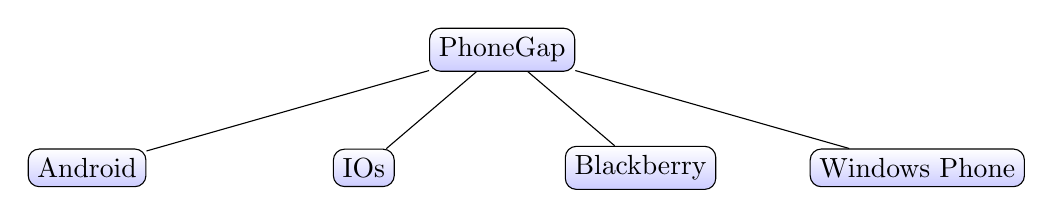
\begin{tikzpicture}[sibling distance=10em,
  every node/.style = {shape=rectangle, rounded corners,
    draw, align=center,
    top color=white, bottom color=blue!20}]]
  \node {PhoneGap}
    child { node {Android} }
    child { node {IOs} }
    child { node {Blackberry} }
    child { node {Windows Phone} };
\end{tikzpicture}
\medskip
\caption{PhoneGap can be compiled into multiple plattoforms.} 
\end{figure}

A disadvantage of developing in PhoneGap is when their is a use of many native features. PhoneGap relies on a development framework and the provided features when building a mobile application. Hence, if the framework is not up to date with the latest new features, the developer will not be able to partake of the features until the framework is updated. If the application is dependent on many native features a hybrid application may have limitations\cite{kohan2015}.   

%\section{Background}\label{section-background}
Android is an operating system used on a wide range of devices. For example a mobile device or tv device. Developing Android applications are written in the programming language Java. 

A hybrid application is a native application which is partially written with web technologies. I.e HTML5, CSS and JavaScript. The part of the application written with web technologies runs within a browsers engine in a so called WebView. A web application running in a browser does not have access to a device native functions such as the bluetooth. However a website running within a WebView can through interaction with the application's native code access a device native functions.

PhoneGap is a framework for developing mobile applications. The code is written with web technologies. The code can be compiled to different platforms, such as Android or IOs specific code. The resulting application is a hybrid application. An example of a mobile application built in PhoneGap is Wikipedia's mobile application.

\section{Lines of code}\label{section-lines-of-code}
Source lines of code is a measurement tool for software development. Source lines of code, also abbreviated as SLOC, is very easy to obtain and is a fairly accurate predictor of development effort\cite[p.~63]{galorath2006}. Measuring SLOC simply means you count the number of lines of code. There are many different ways to measure SLOC, such as Halsted’s approach, function points, physical SLOC and Logical SLOC. 

Physical SLOC is the length of the code excluding comments and blanks. Function points measure functionality and can therefore be measured before the design and coding if the requirement specification is complete\cite[p.~187]{galorath2006}. Halstead’s uses measurable properties such as operands and operators and uses them to identify properties of software. Such as the length, difficulty and effort of the program. Fenton and Bieman describes Halstead’s software science measures as a confused and inadequate measurement. Particularly for other attributes then size\cite[p.~345]{fenton2015}.

Logical SLOC measures the number of statements that carry over one or more physical lines.  For languages with terminators, this can be counted more easily and quickly. As an example, in Java you could count the logical SLOC by counting the number of line-terminating semicolons and closing curly brackets. Logical SLOC represents the programming instructions and data declarations which are converted into executable instructions, i.e. the implementation of the software design. Another positive aspect of of logical SLOC is that it better handles differences in formatting and style conventions than physical SLOC\cite[p.~155]{galorath2006}.

To compare size between two different languages a size conversion table can be used. The table can be used to estimate how many SLOC a program coded in one programming language would have in another language. In the table constructed by Galorath and Evans you can compare a third generation language, a fourth generation language, Ada, Assembly or Pascal\cite[p.~163]{galorath2006}. A third generation language compared to another third generation language would have no conversion rate. 

Source lines of code is a measurement tool for software development. Source lines of code, also abbreviated as SLOC, is very easy to obtain and is a fairly accurate predictor of development effort\cite[p.~63]{galorath2006}. Measuring SLOC simply means you count the number of lines of code. There are many different ways to measure SLOC, such as Halsted’s approach, function points, physical SLOC and Logical SLOC. 

Physical SLOC is the length of the code excluding comments and blanks. Function points measure functionality and can therefore be measured before the design and coding if the requirement specification is complete\cite[p.~187]{galorath2006}. Halstead’s uses measurable properties such as operands and operators and uses them to identify properties of software. Such as the length, difficulty and effort of the program. Fenton and Bieman describes Halstead’s software science measures as a confused and inadequate measurement. Particularly for other attributes then size\cite[p.~345]{fenton2015}.

Logical SLOC measures the number of statements that carry over one or more physical lines.  For languages with terminators, this can be counted more easily and quickly. As an example, in Java you could count the logical SLOC by counting the number of line-terminating semicolons and closing curly brackets. Logical SLOC represents the programming instructions and data declarations which are converted into executable instructions, i.e. the implementation of the software design. Another positive aspect of of logical SLOC is that it better handles differences in formatting and style conventions than physical SLOC\cite[p.~155]{galorath2006}.

To compare size between two different languages a size conversion table can be used. The table can be used to estimate how many SLOC a program coded in one programming language would have in another language. In the table constructed by Galorath and Evans you can compare a third generation language, a fourth generation language, Ada, Assembly or Pascal\cite[p.~163]{galorath2006}. A third generation language compared to another third generation language would have no conversion rate. 

\section{Related work}\label{section-related-work}
% if anyone asks for a deeper research or surroundin topic here the work that we can reco

\iffalse
%not really sure what to do with this section. I think actually might belong in approach
\subsection{Development goals} \label{subsection-development-goals}
Antoher goal is that the mobile application only provides data from native functions. In order to achieve that the web application and mobile application should have a master slave relationship. Where the web application acts as the master and the mobile application as the slave. To get data from the mobiles native functions the web application asks for the data and the mobile application passes the data back.

To enable this master and slave relationship the mobile and web application layer must be able to communicate. Passing commands and data between the layers. It is important the mobile and web application layers has a way of communicating that is developer friendly. 

It is important that the logic of the web application can be written in a general way (non-platform dependant) adapting to the device accessing the web application. So that the same web application code is used for the web application and mobile application.
\fi
%\chapter{Approach}
The first section Research protocol \ref{section-research-protocol} describes the how the investigation has been made. The following section Measuring Lines of Code \ref{section-measuring-lines-of-code} states how the software metric logical lines of code has been used as a measurement of the result. The last section Layer communication \ref{section-layer-communication} explains how the master and slave relationship between the mobile and web application layer are evaluated. 


\section{Research protocol} \label{section-research-protocol}
%How has a practical approach been used?
%%explain how the practical approach is used
%%%our own experiences when developing
%%%producing the mobile applications ourself to get LLOC, uml diagrams and flow diagrams
%%develop a web application
%%use the web application when developing the mobile application

To carry out the investigation proposed in the problem formulation a practical approach has been used. To evaluate and compare the two different methods a mobile application with the same requirements has been developed in each method. Both of the mobile applications make use of the services offered by the same web application.

\subsection{The mobile applications}
The used web application comprises of a single page and is compatible with the web browser Google Chrome. The page displays a form with a text field, a take photo button, an upload photo button, a location button and a submit button, see figure \ref{fig:nativeuml}. To get the image or the location value for the form the user presses the corresponding button. When the upload photo or take photo or location button is pressed the web application uses the Google Chrome’s built in ability to take a photo or upload a photo or get the location.

\begin{figure}[h!]
	\centering
    \includegraphics[width=120mm,natwidth=800,natheight=600]{./img/webAppFrontPage.png}
    \caption{The web app front page displayed in a browser}
    \label{fig:nativeuml}
\end{figure}

The mobile applications consist of two parts. The web application described above and the mobile application encapsulating the web application. The mobile application must encapsulate the web application and display the web application exactly the same way as it is displayed in a browser. The mobile application must use the mobile’s native functions to get the value for the image and the location.

The text field in the web application has no connection to the mobile application layer. 

For taking or uploading the image value in the form the mobile application must an existing image from the image gallery or take a picture using the camera on the phone. The photo passed back to the web application must be in Base64 format. 

The location must be obtained using the mobile’s GPS. 

When the user interacts with the mobile application the interaction must be directly with the web application encapsulated within the mobile application. 

In the project the following were used for developing and testing:
\begin{itemize}
\item Version 21 of the Android SDK when developing using the Android application framework.
\item Apache Cordova CLI version 4.0 when developing using the PhoneGap framework. 
The mobile that was used when testing the mobile applications was a Nexus 5 mobile with the Android version 5.1.1.
\item The web application has been tested in the Google Chrome browser version 44.0.2403.157.
\end{itemize}

\section{Measuring lines of code}\label{section-measuring-lines-of-code}
The resulting mobile applications are measured using a software metric namely logical lines of code. To count logical lines of code Project Code Meter has been used which ignores the following lines of code \cite{project-code-meter2015}

\begin{itemize}
\item Auto-generated code lines.
\item Header files.
\item Ineffective code statements.
\item Pragma compiler directives.
\item Labels.
\item Switch cases are not statements by themselves (so empty "case").
\item Several statements on the same physical line are counted as several LLOC.
\end{itemize}

The mobile application were written in two different programming languages, Java and JavaScript. To compare the measurement result of logical lines of code we use the conversion table described by Galorath and Evans \cite[p.~163]{galorath2006}. JavaScript and Java are both third generation languages and therefore the conversion is roughly 1 to 1. 

The logical lines of code written in the web application layer is also measured in both developing methods. To give an correct result we measured the added logical lines of code that have been written as a result of the mobile application. The resulting lines in the mobile and web application layer is added together to give a total result. 

The logical lines of code in the web application layer is also measured in both developing methods. The resulting lines in the mobile and web application layer is added together to give a total result. 

\section{Layer communication} \label{section-layer-communication}
A prerequisite is that the communication between the mobile application and web application layer has a master and slave relationship. To evaluate this communication a flow diagram of the web layer sending a request for native data and the mobile application layer responding with data is constructed. The flow diagram acts as a suggestion in how developer friendly the communication is combined with our personal developing experiences.
%\chapter{Evaluation}	
The evaluation is divided into two sections, one for each development method used. In each section, the developed application, it's structure and functionality is presented, followed by the results of the code evaluation. 

\section{Native android} \label{android}
The developed native application can be cloned from Github at [..], also a compressed version of all source code used in the thesis can be found at [..]. An overview of the application structure and functionality follows in section ~\ref{sec:nativestructure}. 

\subsection{Application structure} \label{sec:nativestructure}
A UML-diagram representing the Android application can be seen in figure ~\ref{fig:nativeuml}, with the classes summarized below.

\begin{description}
	\item[MainActivity] is the main class of the program, containing Android-specific code related to startup logic, activities to be started and shutdown of the application. It also serves as a messenger, sending back data from native functions upon completion.
	
	\item[IntentFactory] provides intents for native functions 
	
	\item[AndroidHardware] handles hardware related logic, such as file creation.
	
	\item[Bridge] serves as a bridge between the native application and web. When a native function is requested, Bridge requests the corresponding Intent from IntentFactory, and creates a Callback of the corresponding type. The Intent is sent to MainActivity for execution, and the Callback is stored in MainActivity.
	
	\item[WebViewDataSender] is the class communicating back to the web application by invoking javascript-functions in the browser.
	
	\item[JsInterface] is exposed to the web application as a JavaScriptInterface and acts as a receiver for function calls from the web application. Whenever native functionality is needed, the javascript in the web application can call upon it's methods. JsInterface forwards the function calls to Bridge, which in turn, contains the logic for each function.
	
	\item[Callback] contains logic specifying how to send results from a native function back to the web application.
	
	\begin{description}
		\item[ImageCallback] is used when the web application requests an image from the camera.
		
		\item[ImagePickCallback] is used when the web application requests an image from the gallery.
		
	\end{description}
	\item[UniqueInteger] is used by MainActivity when storing callbacks. An unique integer is used as an id for an Intent and its related callback. Upon completion of an Intent, the Callback with the same id is executed.
	
\end{description}

\begin{figure}[h!]
	\centering
    \includegraphics[width=120mm,natwidth=800,natheight=600]{./img/polluxuml.png}
    \caption{Structure of the android application}
    \label{fig:nativeuml}
\end{figure}

In order to simplify development of the web application with support for both web browsers and the Android application, part of the logic follows the adapter pattern. The business logic of the web application stays the same, and only the communication with the unit (web browser or application), for example when uploading a picture, differs. Figure ~\ref{fig:nativewebuml} displays the basic structure of the web application. 

\begin{figure}[h!]
	\centering
    \includegraphics[width=60mm,natwidth=400,natheight=300]{./img/androidwebuml.png}
    \caption{Structure of the web application}
	\label{fig:nativewebuml}
\end{figure}

A more detailed view of the program flow when the web application requests an image can be seen in figure ~\ref{fig:nativeflow}, further explained below.
\begin{figure}[h!]
	\centering
    \includegraphics[width=120mm,natwidth=800,natheight=600]{./img/androidfunctionflow.png}
    \caption{Function flowchart, single call from web application}
    \label{fig:nativeflow}
\end{figure}
\begin{enumerate}
	\item User action invokes a request for an image from the mobile camera
	\item Current device adapter (AndroidDeviceAdapter) calls requestCamera on JsInterface, with the function name of the preferred callback function as argument
	\item JsInterface forwards the function call to Bridge
	\item Bridge creates the corresponding Intent and Callback, and calls processIntent on MainActivity with Intent and Callback as arguments
	\item MainActivity Creates gets a unique id from UniqueInteger, stores the callback in a hashmap with the id as key, and starts the intent with the id as requestcode.
	\item Camera application starts
	\item When user takes a picture, MainActivity gets notified by the Android system, pulls the Callback with the same id as the processed Intent, and forwards the callback and resulting image data to Bridge through processCallback
	\item Bridge executes the callback which in turn calls sendData on WebViewDataSender, with the image data and callback name as arguments
	\item WebViewDataSender executes the javascript callback function in the browser window
	\item The captured image is displayed to the user in the browser
\end{enumerate}

\subsection{Code evaluation}
Evaluation of the developed application was performed as described in [...], and a summary of the results  can be seen in table ~\ref{tab:lloc1}.

\begin{table}[!htb]
    \centering
        \begin{tabular}{lrc}\hline
			\end{tabular}
    \caption{Code evaluation - Native application}\label{tab:lloc1}
\end{table}

\section{PhoneGap}
The application developed in PhoneGap can 

\subsection{Application structure}

\begin{figure}[h!]
	\centering
    \includegraphics[width=120mm,natwidth=800,natheight=600]{./img/phonegapuml.png}
    \caption{Structure of the phonegap application}
    \label{fig:phonegapuml}
\end{figure}

\begin{figure}[h!]
	\centering
    \includegraphics[width=60mm,natwidth=400,natheight=300]{./img/phonegapwebuml.png}
    \caption{Structure of the web application}
        \label{fig:phonegapwebuml}
\end{figure}

\begin{figure}[h!]
	\centering
    \includegraphics[width=120mm,natwidth=800,natheight=600]{./img/phonegapfunctionflow.png}
    \caption{Function flowchart, single call in web application}
\end{figure}

\subsection{Code evaluation}
Evaluation of the developed application was performed as described in [...], and a summary of the results  can be seen in table ~\ref{tab:lloc2}.

\begin{table}[!htb]
    \centering
        \begin{tabular}{lrc}\hline
			\end{tabular}
    \caption{Code evaluation - PhoneGap application}\label{tab:lloc2}
\end{table}
%\chapter{Discussion} \label{ch:discussion}
The problem formulation in section~\ref{sec:problem-formulation} can be summarized to:
What are the differences in code structure and development effort for two different development methods for encapsulating an existing web application in a mobile application to utilize native functions?

Our results show that developing such a mobile application in the PhoneGap framework requires less development effort than in the Android framework. A reason for this might be that calls to native functions are handled on a higher abstraction level. Another reason is that 10 classes were used in the Android framework compared to an eqvuivalent to 4 classes in the PhoneGap framework.

The structure that we suggested in the Android framework is modular, separating creation of a request for a native function, handling of the data passed back from the request and communication with the web application layer. The PhoneGap framework also separates the communication with the web application layer, but a request for a native function and handling of the data passed back is located in the same file. 

The mobile application developed in the PhoneGap framework has fewer steps from receiving a request from the web application layer to pass the data back, see flowchart~\ref{fig:nativeflow} and~\ref{fig:phonegapflow}. This suggests that the application developed in the PhoneGap framework has a less complex structure then the application developed in Android framework.

The PhoneGap framework has a higher abstraction level of calls to native functions. That allows for fewer logical lines of code, but there is a downside. The downside is that one has less freedom in terms of customizing the behavior. The loss of freedom makes no difference for a simple mobile application such the one developed, but as Kohan and Montanez points out for a more complex application it might be a problem, see section~\ref{subsec:phonegap}. 

In the Android framework there is a closer relation to the Android System/Hardware, however this comes with a requirement of boilerplate code. That is one of the reasons that the mobile application that was developed in the Android framework had more than double the logical lines of code. This closer relation means that the developer can have a better control over the application lifecycle. The closer relation also means that basic knowledge of Android is needed. If the developer has no prior knowledge of Android this means a starting cost. 

Encapsulating the web application front-end in the PhoneGap framework was made at the cost of a security flaw. The web application front-end was encapsulated by use of an IFrame. To be able to use an IFrame the web applications X-Frame-Options response header was removed which makes it possible to use the web application for ClickJacking, see section~\ref{sec:iframe}. 

There are other ways of encapsulating the front-end of a web application in the PhoneGap framework than by using an IFrame. Another way would be to use a plugin that is available in the PhoneGap API called inAppBrowser. By using inAppBrowser a web page can be loaded into the mobile application and the mobile application layer can execute the web page’s JavaScript functions. If the web page would like to send a request to the mobile application layer the mobile application layer can listen to such requests by the use of polling.  This could be an alternative to using an IFrame that would not expose the web application to be used for ClickJacking. 

To compare the development effort the software metric logical lines of code were used. Logical lines of code were chosen since it is easy to understand, measurable between two programming languages and simple to calculate. Other ways of measuring lines of code or other software metrics could have been used to measure development effort or other properties. To measure more properties and also measure development effort in other ways would have provided a more nuanced result and a fuller picture. For example Halsted's approach, described in section~\ref{sec:lines-of-code}, could have been used to measure the development effort. Another property that could have been measured would have been cyclomatic complexity. Cyclomatic complexity measures the number of linearly independent paths through a program’s source code. 

The result of this study is drawn from one small and simple project. This makes it hard to draw any conclusions about using the two development methods for medium and large projects. It raises the question whether developing in the PhoneGap framework in bigger projects or using more advanced features would still score lower in development effort. One interesting question would be whether the proposed structure in the development methods provide a good bone structure for more complex projects? Or would the structure crumble? The measurement and proposed structure is based on this single project. To get a more reliable result it would be interesting to collect data from a number of projects where a mobile application, encapsulating an existing web application, has been developed in both development methods.

The structure we proposed in the web application, to be able to run both in a web browser and in a mobile application, makes use of the adapter pattern. This makes it easy to further extend web applications functionality. If a new function has no connection to native functionality, such as an animation, the function can be implemented as if the mobile application did not exist. When new functionality is needed which includes native functionality, such as getting information from the accelerometer, then the web application need at least three functions. The first function is needed to make the request to the mobile application and a second function is needed which determines the functionality on a browser. Finally a function which handles the data which is passed back from the request. 

%\chapter{Conclusions}
Slutsatser (Conclusions) bör sammanfatta dina slutsatser och redogöra för möjliga förbättringar och eventuella rekommendationer.
\begin{thebibliography}{9}

\bibitem{galorath2006}
Daniel D. Galorath and Michael W. Evans, \emph{Software Sizing, Estimation, and Risk 	Management}, Auerbach Publications, Taylor and Francis Group, 2006.
  
\bibitem{fenton2015}
Norman Fenton, Queen Mary University of London, UK, James Bieman, Colorado State University, Fort Collins, USA, \emph{Software Metrics: A Rigorous and Practical Approach}, CRC Press, Taylor and Francis Group, 3rd edition, 2015
  
\bibitem{kohan2015}
Bernard Kohan and Joseph Montanez,
\emph{Native vs Hybrid/PhoneGap App Development Comparison},
  \url{http://www.comentum.com/phonegap-vs-native-app-development.html},
  Comentum, San Diego,
  January 26, 201EffectiveUI5
  
\bibitem{harris2010}
	Online survey from Harris Interactive on behalf of EffectiveUI,
	United States,
September 30 - October 4, 2010

\bibitem{pcm2015}
	Project Code Meter,
	\url{www.projectcodemeter.com},
September 8, 2015

\bibitem{pcmlloc2015}
	Project Code Meter - Logical Lines of Code,
	\url{http://www.projectcodemeter.com/cost_estimation/help/GL_lloc.htm},
September 8, 2015

\end{thebibliography}
%
% example exists at http://www.texample.net/tikz/examples/marketing-distribution-channel/
\begin{figure}
\centering
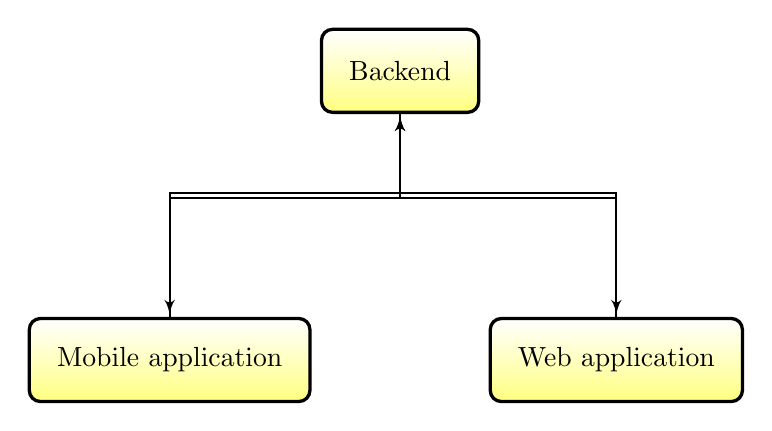
\begin{tikzpicture}[node distance=1cm, auto]  
\tikzset{
    mynode/.style={rectangle,rounded corners,draw=black, top color=white, bottom color=yellow!50,very thick, inner sep=1em, minimum size=3em, text centered},
    myarrow/.style={->, >=latex', shorten >=1pt, thick},
    mylabel/.style={text width=7em, text centered} 
}  
\node[mynode] (backend) {Backend};  
\node[below=3cm of backend] (dummy) {}; 
\node[mynode, left=of dummy] (mobile) {Mobile application};  
\node[mynode, right=of dummy] (web) {Web application};

\draw[myarrow] (backend.south)  -- ++(0,-1) -|  (mobile.north);
\draw[myarrow] (mobile.north)  -- ++(0,1.506) -|  (backend.south);
\draw[myarrow] (backend.south)  -- ++(0,-1) -|  (web.north);
\draw[myarrow] (web.north)  -- ++(0,1.506) -|  (backend.south);
% There is a slight overlap of the arrows with the (manufacturer) south edge
% because creating the offset in another way didn't compile. 

\end{tikzpicture} 
\medskip
\caption{Seperate mobile and web application connected with a common backend.} 
\end{figure}
\begin{figure}
\centering
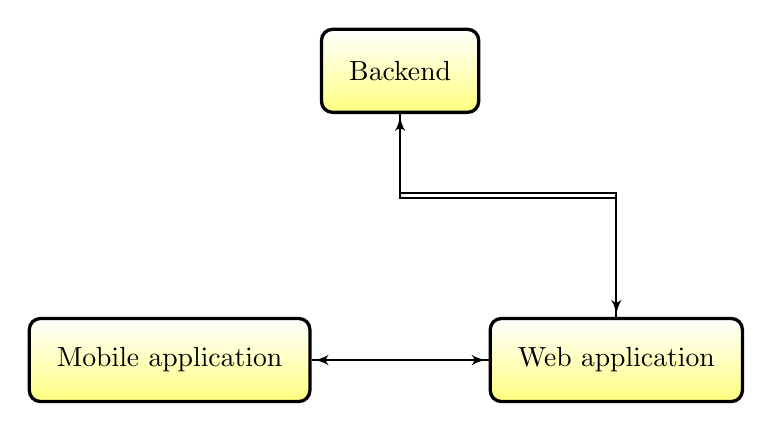
\begin{tikzpicture}[node distance=1cm, auto]  
\tikzset{
    mynode/.style={rectangle,rounded corners,draw=black, top color=white, bottom color=yellow!50,very thick, inner sep=1em, minimum size=3em, text centered},
    myarrow/.style={->, >=latex', shorten >=1pt, thick},
    mylabel/.style={text width=7em, text centered} 
}  
\node[mynode] (backend) {Backend};  
\node[below=3cm of backend] (dummy) {}; 
\node[mynode, left=of dummy] (mobile) {Mobile application};  
\node[mynode, right=of dummy] (web) {Web application};

\draw[myarrow] (backend.south)  -- ++(0,-1) -|  (web.north);
\draw[myarrow] (web.north)  -- ++(0,1.506) -|  (backend.south);
\draw[myarrow] (web.west)  -- (mobile.east);
\draw[myarrow] (mobile.east)  -- (web.west);
% There is a slight overlap of the arrows with the (manufacturer) south edge
% because creating the offset in another way didn't compile. 

\end{tikzpicture} 
\medskip
\caption{Seperate mobile and web application connected with a common backend.} 
\end{figure}
% example exists at http://www.texample.net/tikz/examples/tree/
\begin{figure}
\centering
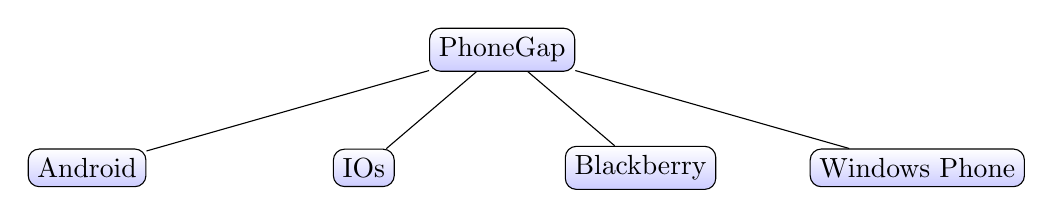
\begin{tikzpicture}[sibling distance=10em,
  every node/.style = {shape=rectangle, rounded corners,
    draw, align=center,
    top color=white, bottom color=blue!20}]]
  \node {PhoneGap}
    child { node {Android} }
    child { node {IOs} }
    child { node {Blackberry} }
    child { node {Windows Phone} };
\end{tikzpicture}
\medskip
\caption{PhoneGap can be compiled into multiple plattoforms.} 
\end{figure}
\end{document}